\chapter{Turtlemint Projects with Django}

Majority of the Turtlemint codebase is written in Java. Hence, introduction
of Python and Django in specific was very new to the team. As a part of the
project I was working on two of their major projects namely, Turtlemint
Assistant and MintAcademy. Both of these applications are deployed on
production and are completely written in Django.

\section{Turtlemint Assistant Project}
The Turtlemint Assistant Project is one of the newest projects Turtlemint as
developed. Me along with other interns are one of the core backend developers
for this project. This project was written from scratch and involved all
development processes discussed in last chapter.

The development processed involved majorly involved following activities:

\begin{itemize}
    \item Understanding the existing database
    \item Replicating the existing database in relational model
    \item Starting a new Django project
    \item Developing the project to solve all requirements
    \item Take feedback from managers and project leads
    \item Testing the application
    \item Preparing unittests and integration tests
    \item Deploying application on staging server and then on production
    \item Solving issues, releasing bug fixes
    \item Feedback from users and adapting to their requirements
\end{itemize}

\subsection{The primary objective}
The primary objective of the project was to let the data team to conveniently
update the insurer data in database. Since Turtlemint is an insurance company
and acts as a broker between the insurance providers and customers, it has to
record all insurer data in order to punch insurance policies on their behalf.
This data is updated very frequently by the insurers and hence Turtlemint too
has to adpat to those changes quickly to avoid punching wrong policies.

This was then acted upon us in order to provide them a common platform to
handle database updates with a sophisticated yet simple user interface and
reliable and stable system.

\subsection{The features}
The application provides a ton lot of features assisting the team with their
updates. Here is a summary of the features we developed:

\begin{itemize}
    \item Social authentication -- Login through Google

    The user can simply login via his Google account in Turtlemint assistant.
    The benefit being the user don't have to remember its username, password.
    Also, the Google only permits users with Turtlemint issued domain emails
    to login and proceed towards the application.
    \begin{figure}
        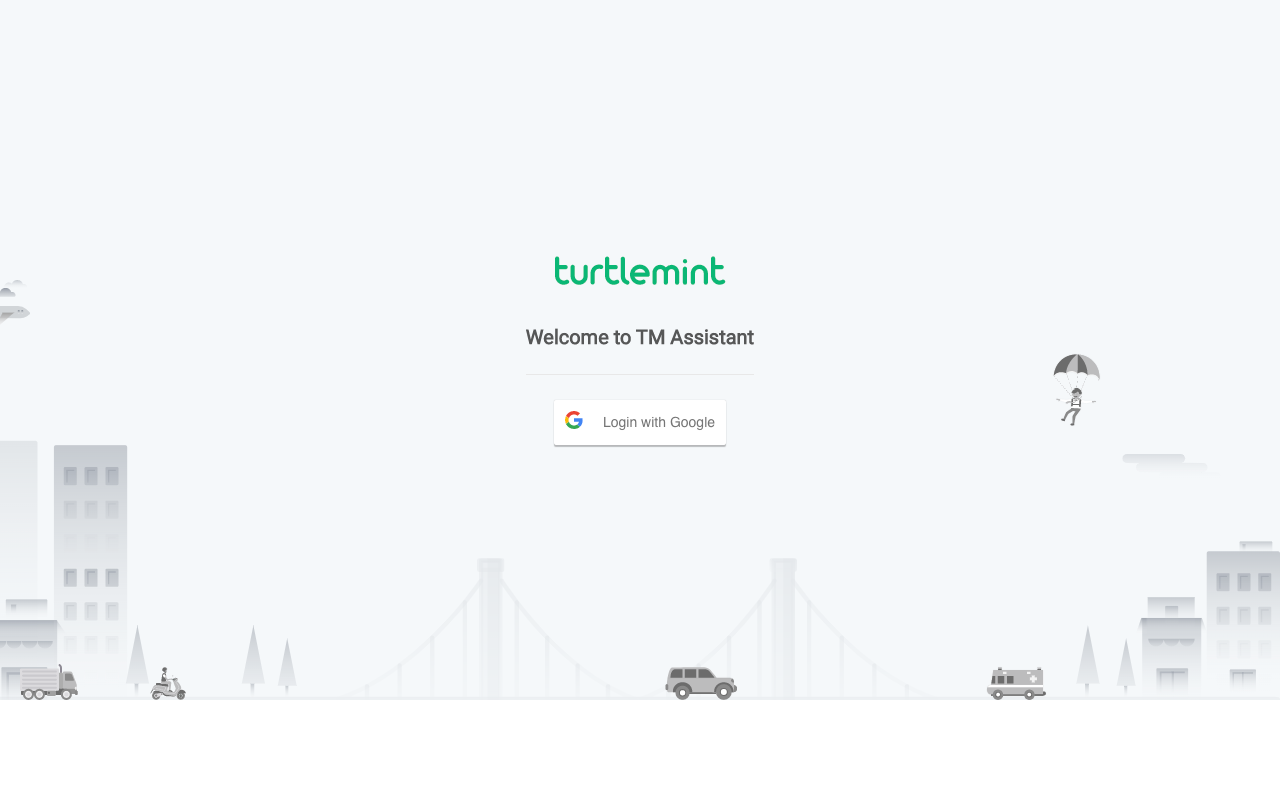
\includegraphics[width=\textwidth]{ch5/tap_social_auth.png}
        \caption{The Turtlemint assistant social auth screen}
    \end{figure}

    \item The insurer-wise mapping data stats

    There is a separate screen for the user to check which data is yet to be
    processed or \textit{mapped} to the Turtlemint database. This stats are
    displayed insurer-wise are are extremely helpful in determining which
    insurer data needs attention and to track overall progress.
    \begin{figure}
        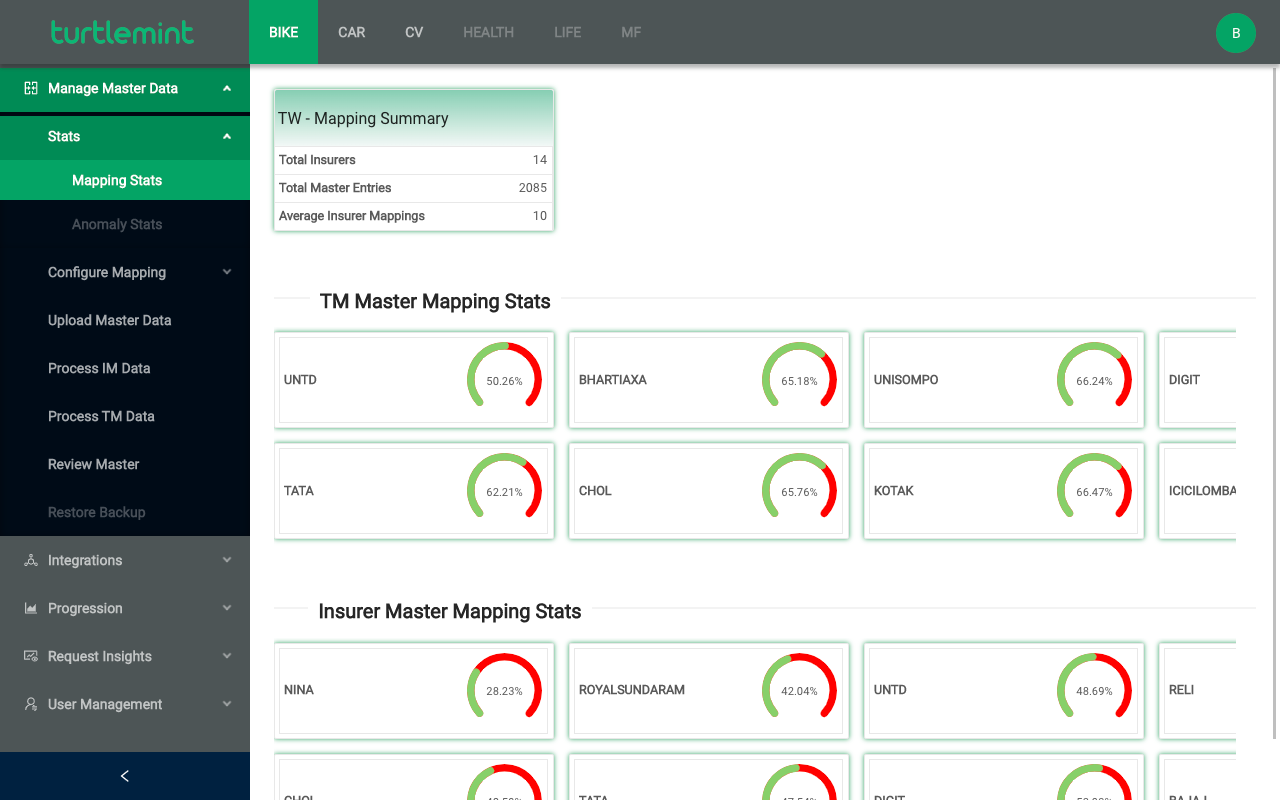
\includegraphics[width=\textwidth]{ch5/tap_stats.png}
        \caption{The Turtlemint assistant stats screen}
    \end{figure}

    \item Upload raw insurer file and calculate changes.

    The user can simply upload the received file from the insurer and let
    the application detect all new changes received from the file. Then the
    user only needs to work on those new changes instead of going through all
    changes.
    \begin{figure}
        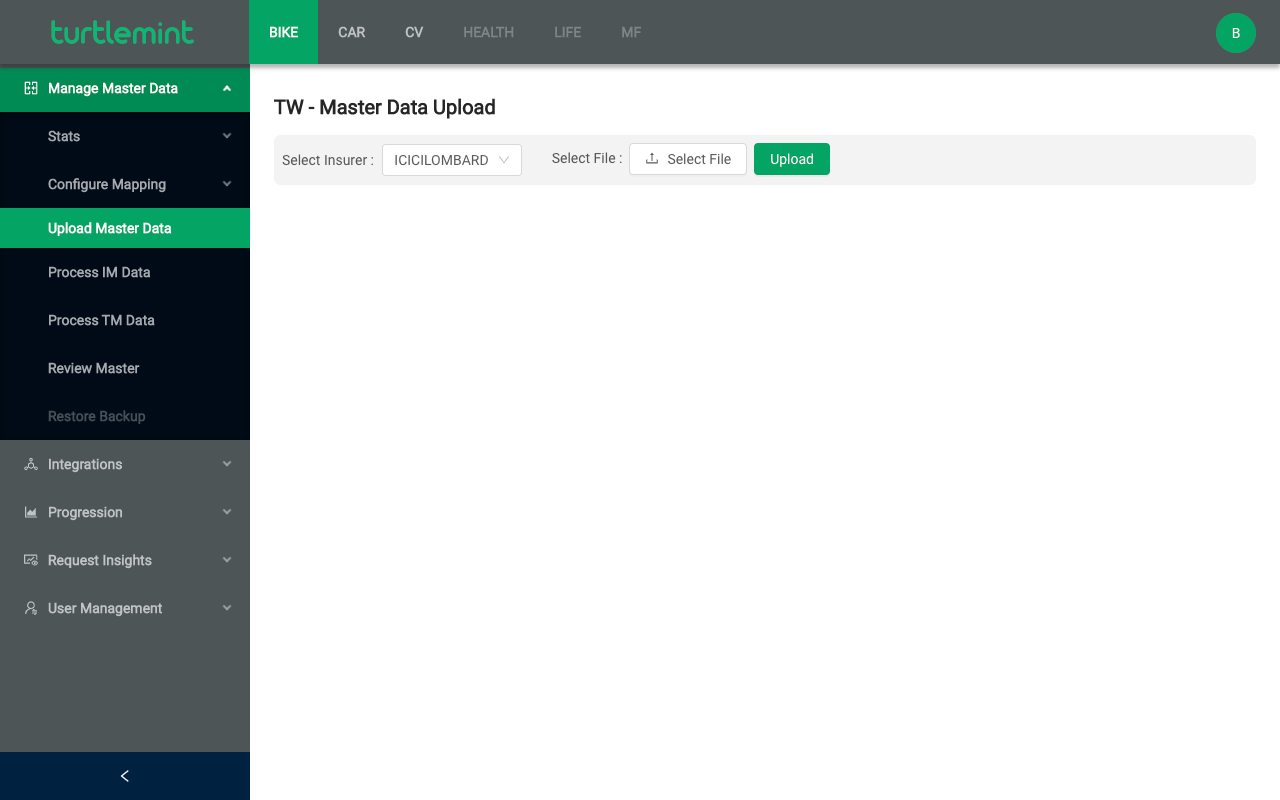
\includegraphics[width=\textwidth]{ch5/tap_upload_file.png}
        \caption{The Turtlemint assistant upload screen}
    \end{figure}

    \item Process all data and take suitable action

    The data is distributed between various type of changes and the user can
    work on them individually wither by accepting or rejecting new changes.
    This is split across all insurers and hence multiple users can work on
    set of different insurers at the same time, optimizing the overall process.
    \begin{figure}
        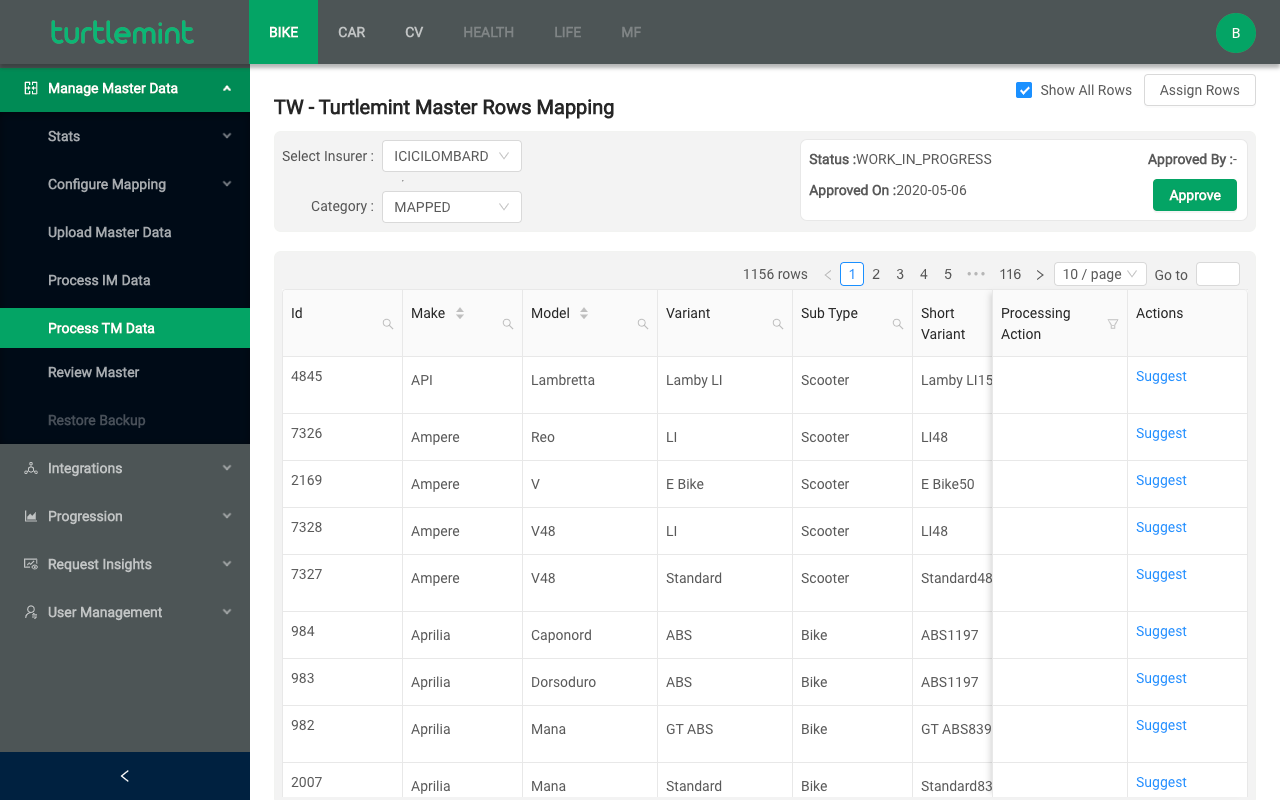
\includegraphics[width=\textwidth]{ch5/tap_data_work.png}
        \caption{The Turtlemint assistant data screen}
    \end{figure}

    \item Suggest records to be mapped with turtlemint datbase

    The insurer data can be mapped with the Turtlemint database making them
    as an active entity in the insurance issuing process. This can be easily
    done via the application is extremely helpful since the user doesn't have
    to find the record's equivalent entry in Turtlemint database manually.
    \begin{figure}
        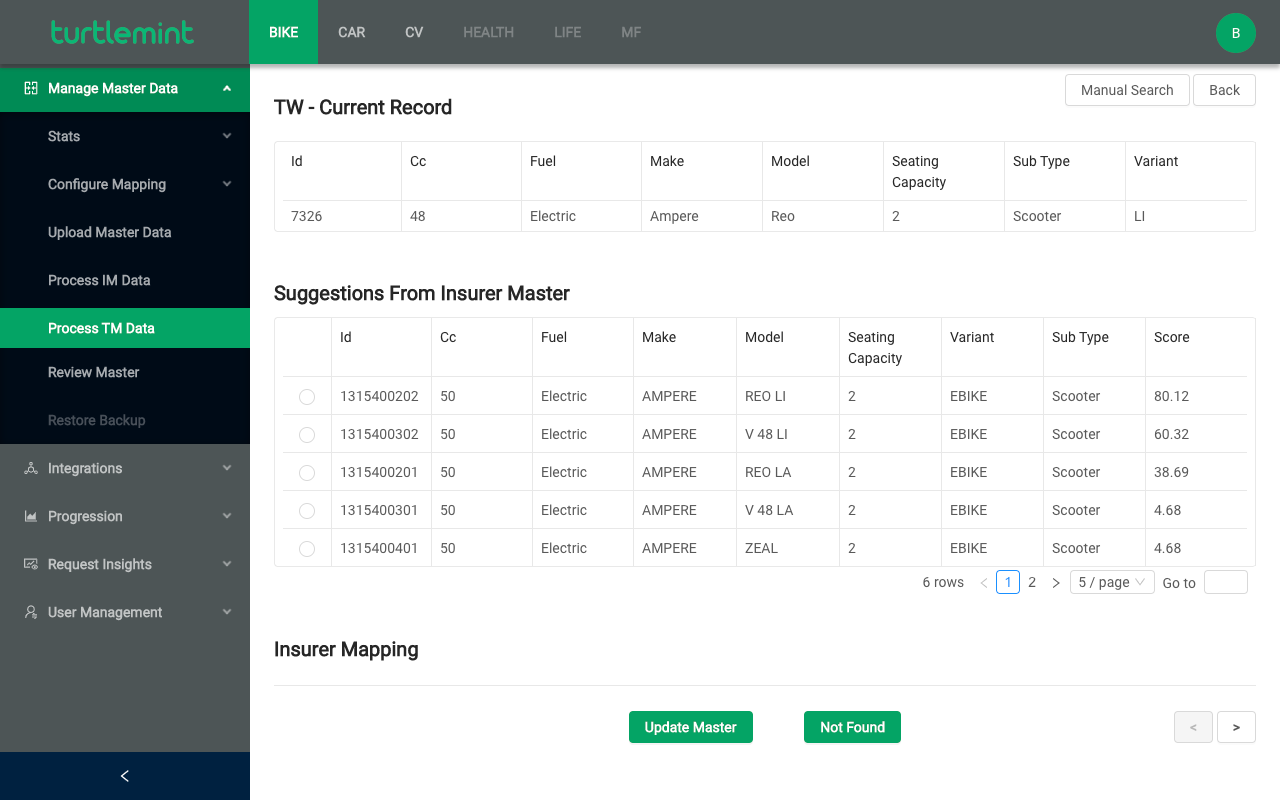
\includegraphics[width=\textwidth]{ch5/tap_suggest.png}
        \caption{The Turtlemint assistant suggest screen}
    \end{figure}
\end{itemize}

\section{MintAcademy}

MintAcademy is an Learning Management Software (LMS) developed as a SaaS
(Software as a Service) platform for its tenants. The MintAcademy was
originally written using GCP (Google Cloud Platform), GAE (Google App Engine)
and NDB Storage. With the rising issues and cost reduction, it was and still
is being re-written in Django. I'm one of the core developers involved in this
migration. Until now, most of the core functionality is already migrated
and is expected to go live in the month of June, 2020.

The current implementation uses GCP extensively and uses all of its features.
It is currently live on production server and is serving to thousands of users
at the moment.
